\documentclass[12pt,a4paper]{article}
\usepackage[utf8]{inputenc}
\usepackage[T1]{fontenc}
\usepackage{amsmath}
\usepackage{amssymb}
\usepackage{graphicx}
\usepackage{a4wide}
\usepackage{caption}
\usepackage{booktabs}
\usepackage{indentfirst}
\usepackage{anyfontsize}
\usepackage[hidelinks]{hyperref}
\title{Predicting the penguin species}
\author{Oldřich Šmehlík, Artem Sorokin, Kryštof Dostál, Jan Jiran, Jakub Chládek}
\usepackage[sfdefault]{roboto}

\usepackage[
backend=biber,
style=iso-authoryear,%iso-numeric,
sorting=ynt
]{biblatex}
\addbibresource{citation.bib}

\begin{document}
\maketitle

%\begin{abstract}
%V této eseji
%\end{abstract}

\section{Introduction}

In course 4IT439 Data-X – applied data analytics models in real world tasks
taught at Faculty of Informatics and Statistics, Prague University
of Economics and Business in summer semester 2023,
the course instructors assigned us to write a term paper on predicting penguin species.
This document is the result of our work.

\section{Problem Definition}

The target is to predict the species of penguin (multi-class classification), based on a popular, slightly modified (for the purpose of this exercise) Palmer Penguins dataset.
The goal of this project is to create, optimize and evaluate several models to do so. The success of the models will be measured in prediction accuracy. Since the dataset is very small, calculation time is not a suitable measurement.
The dataset does need some data preparation (such as treating NaN values, duplicates etc.). The preparation is part of this project, and will include replacing missing values, omitting unuseful attributes and other modifications.

\section{Data Understanding}

\subsection{Dataset Introduction}

The original dataset (without modifications) comes from a study (\cite{10.1371/journal.pone.0090081}) and can also be publicly found at the following URL: 

\medskip
\noindent
\url{https://gist.github.com/slopp/ce3b90b9168f2f921784de84fa445651}
\medskip

\noindent
The dataset provided for this project was however slightly changed for the purpose of learning to treat certain situations. 

\subsection{Dataset Content}

Our dataset contains $363$ rows and $8$ columns:

\begin{itemize}
\item $1$ column with target variable (\texttt{species})
\item $7$ columns with possible input features (\texttt{island}, \texttt{bill\_length\_mm}, \texttt{bill\_depth\_mm}, \texttt{flipper\_length\_mm}, \texttt{body\_mass\_g}, \texttt{sex}, \texttt{year})
\item $5$ columns with numerical values (\texttt{bill\_length\_mm}, \texttt{bill\_depth\_mm}, \texttt{flipper\_length\_mm}, \texttt{body\_mass\_g}, \texttt{year}), out of these $4$ contains floating numbers (\texttt{bill\_length\_mm}, \texttt{bill\_depth\_mm}, \texttt{flipper\_length\_mm}, \texttt{body\_mass\_g}) and $1$ contain integer number (\texttt{year})
\item $3$ columns with categorical values (\texttt{species}, \texttt{island}, \texttt{sex})
\end{itemize}

The representation of the target variable (\texttt{species}) is:

\begin{itemize}
\item \texttt{Adelie} -- $160$ occurences
\item \texttt{Gentoo} -- $124$ occurences
\item \texttt{Chinstrap} -- $79$ occurences
\end{itemize}

As we can see, the classes are imbalanced. To solve this, we have decided to use oversampling using SMOTE method to solve class imbalance in our case.

\subsection{Missing values}

\begin{figure}[h]
	\centering
	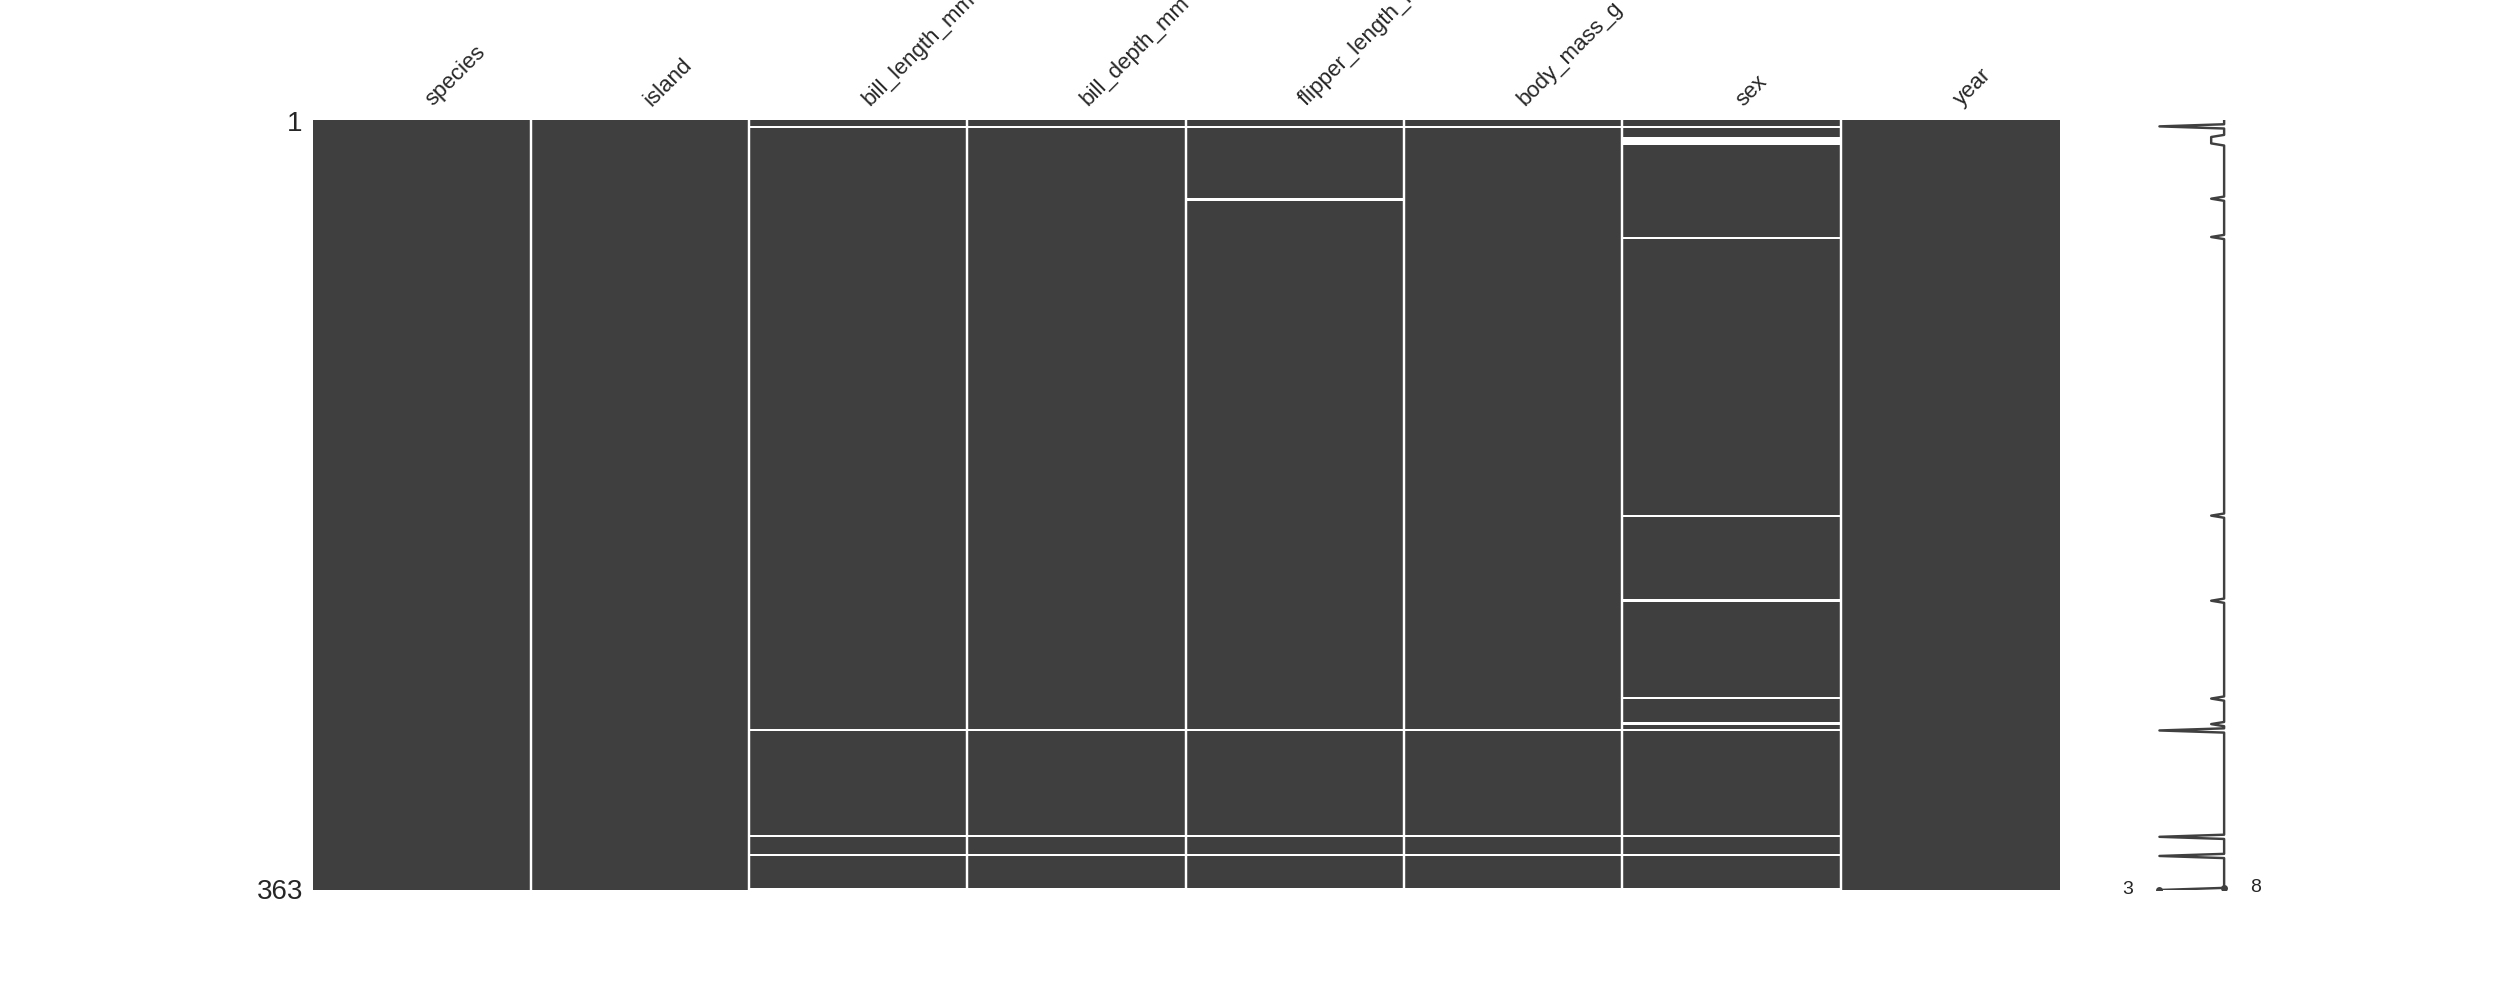
\includegraphics[width=1.0\linewidth]{fig_missing_values}
	\caption{Placement of missing values in dataset}
	\label{fig:figmissingvalues}
\end{figure}

As we can see in Figure \ref{fig:figmissingvalues},
our dataset contains a small amount of missing values in columns \texttt{bill\_length\_mm}, \texttt{bill\_depth\_mm}, \texttt{flipper\_length\_mm}, \texttt{body\_mass\_g}, \texttt{sex}.
The gender (sex) of the penguin is missing quite often. This is probably due to the fact that telling the sex of the penguin is often difficult - sometimes even for the penguins. It is a popular theory that penguins have the highest percentage of same sex couples (up to 28\% according to some studies), because most species mate for life and can “make a mistake”, when picking their mate.
One of the common ways to determine the penguin sex is to measure it’s bill (beak) - male bills are often slightly larger.

\subsection{Correlations}

Correlation between input features is shown textually in Table \ref{tbl:correlations}
and visually in Figure \ref{fig:figcorrelation}.
As we can see, the most correlated features are \texttt{body\_mass\_g} and
\texttt{flipper\_length\_mm} with correlation value of $0.86$.

\begin{table}[h]
\centering \tiny

\begin{tabular}{|l|r|r|r|r|r|}
	\hline
	{} &  bill\_length\_mm &  bill\_depth\_mm &  flipper\_length\_mm &  body\_mass\_g &      year \\
	\hline
	bill\_length\_mm    &        1.000000 &      -0.219291 &           0.639585 &     0.578546 &  0.050733 \\
	bill\_depth\_mm     &       -0.219291 &       1.000000 &          -0.586423 &    -0.479516 & -0.090926 \\
	flipper\_length\_mm &        0.639585 &      -0.586423 &           1.000000 &     0.869749 &  0.201139 \\
	body\_mass\_g       &        0.578546 &      -0.479516 &           0.869749 &     1.000000 &  0.082095 \\
	year              &        0.050733 &      -0.090926 &           0.201139 &     0.082095 &  1.000000 \\
	\hline
\end{tabular}
\captionof{table}{Correlations}\label{tbl:correlations}
\end{table}

\begin{figure}[h]
	\centering
	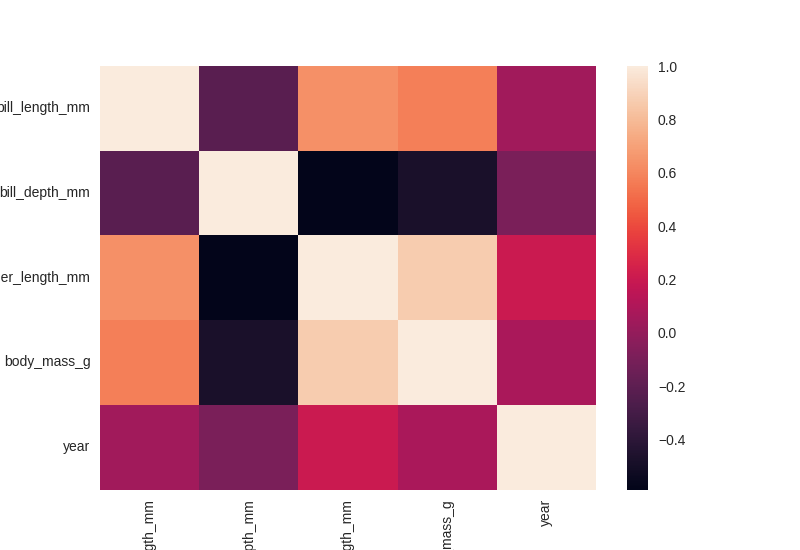
\includegraphics[width=0.7\linewidth]{fig_correlation}
	\caption{Correlations}
	\label{fig:figcorrelation}
\end{figure}

\section{Data Preparation}

The \texttt{year} column was found not suitable for predicting, since it says little about the penguin, changes in the future and potentially degrades the quality of the predictions. Therefore it will be omitted, and only physical attributes of the penguin and the location where it was found (\texttt{island}) will be used.

Afterwards, 13 duplicates are removed, rows with more than 5 NaN values are also deleted (since they can hardly provide enough valuable information for accurate prediction) and datatypes are converted (\texttt{species}, \texttt{island}, \texttt{sex} to categorical).

For missing sex values, a Random Forest model is created to replace them. For the other missing values, a mean value of the other ones is used for replacement.

We split dataset into train (80\% of the dataset) and test (20\% of the dataset) parts using split stratified by our target variable.
We do oversampling using SMOTE method on train part.
We also standard scale numerical columns and one hot encode categorical columns.

\section{Data Visualization}

\subsection{Island habitability}

\begin{figure}[h]
	\centering
	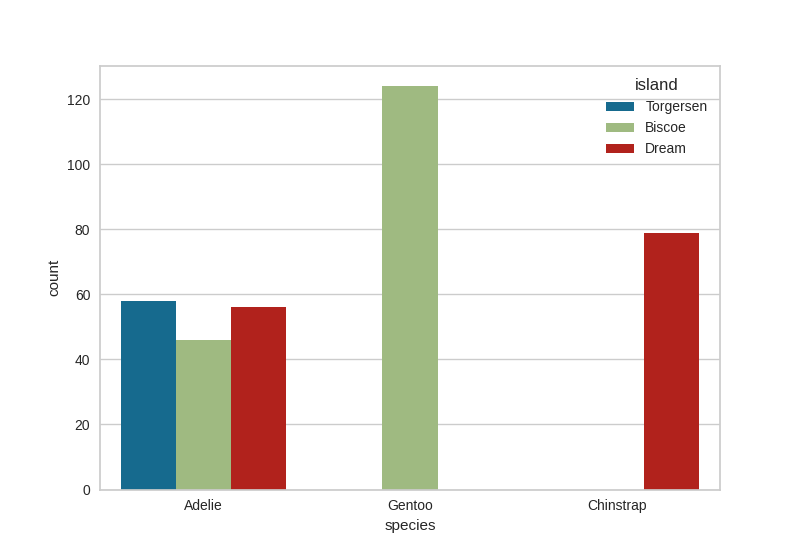
\includegraphics[width=0.8\linewidth]{fig_island_habitability}
	\caption{Island habitability}
	\label{fig:fig_island_habitability}
\end{figure}

First, we used the countplot from seaborn to demonstrate the separation of penguins on the three islands.
This is shown on Figure \ref{fig:fig_island_habitability},
Adelie species inhabit all three islands, but Gentoo and Chinstrap are separated.
Gentoo lives on Biscoe Island.
Chinstrap lives on Dream Island.
It follows that we need to find patterns in our data with which we can distinguish Adelie from the other species.

\subsection{Outliers}

The next visualization serves to identify outliers. Boxplots do an excellent job with this task. The boxplot edges correspond to 1 and 3 quartiles, the whisker tips represent the minimum and maximum values, and the points outside the graph are outliers. We can see from the Figure \ref{fig:boxplots} that the outliers are present, but their number is minimal.

\begin{figure}[h]
	\centering
	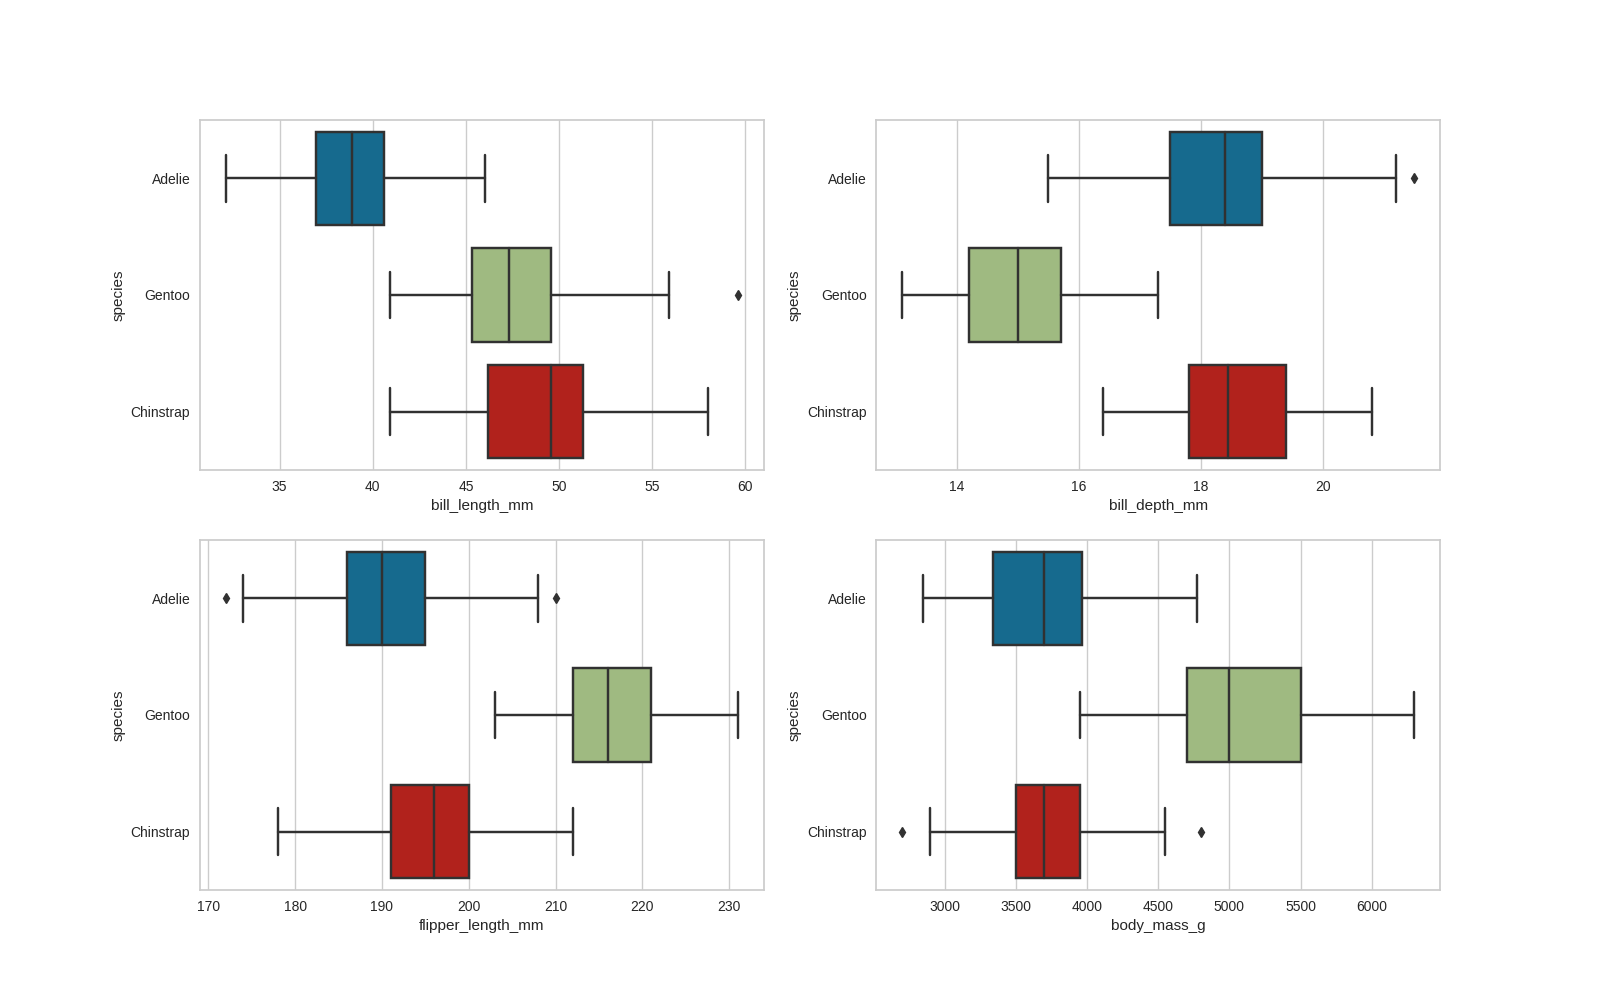
\includegraphics[width=1.0\linewidth]{fig_boxplots}
	\caption{Boxplots}
	\label{fig:boxplots}
\end{figure}

\subsection{Pairplots}

By using the sns.pairplot graph, which builds a scatter plot matrix, we can see how well the Gentoo species separates on the dot plot between the \texttt{bill\_depth\_mm} and \texttt{body\_mass\_g} features. This is shown on Figure \ref{fig:pairplots}.

\begin{figure}[h]
	\centering
	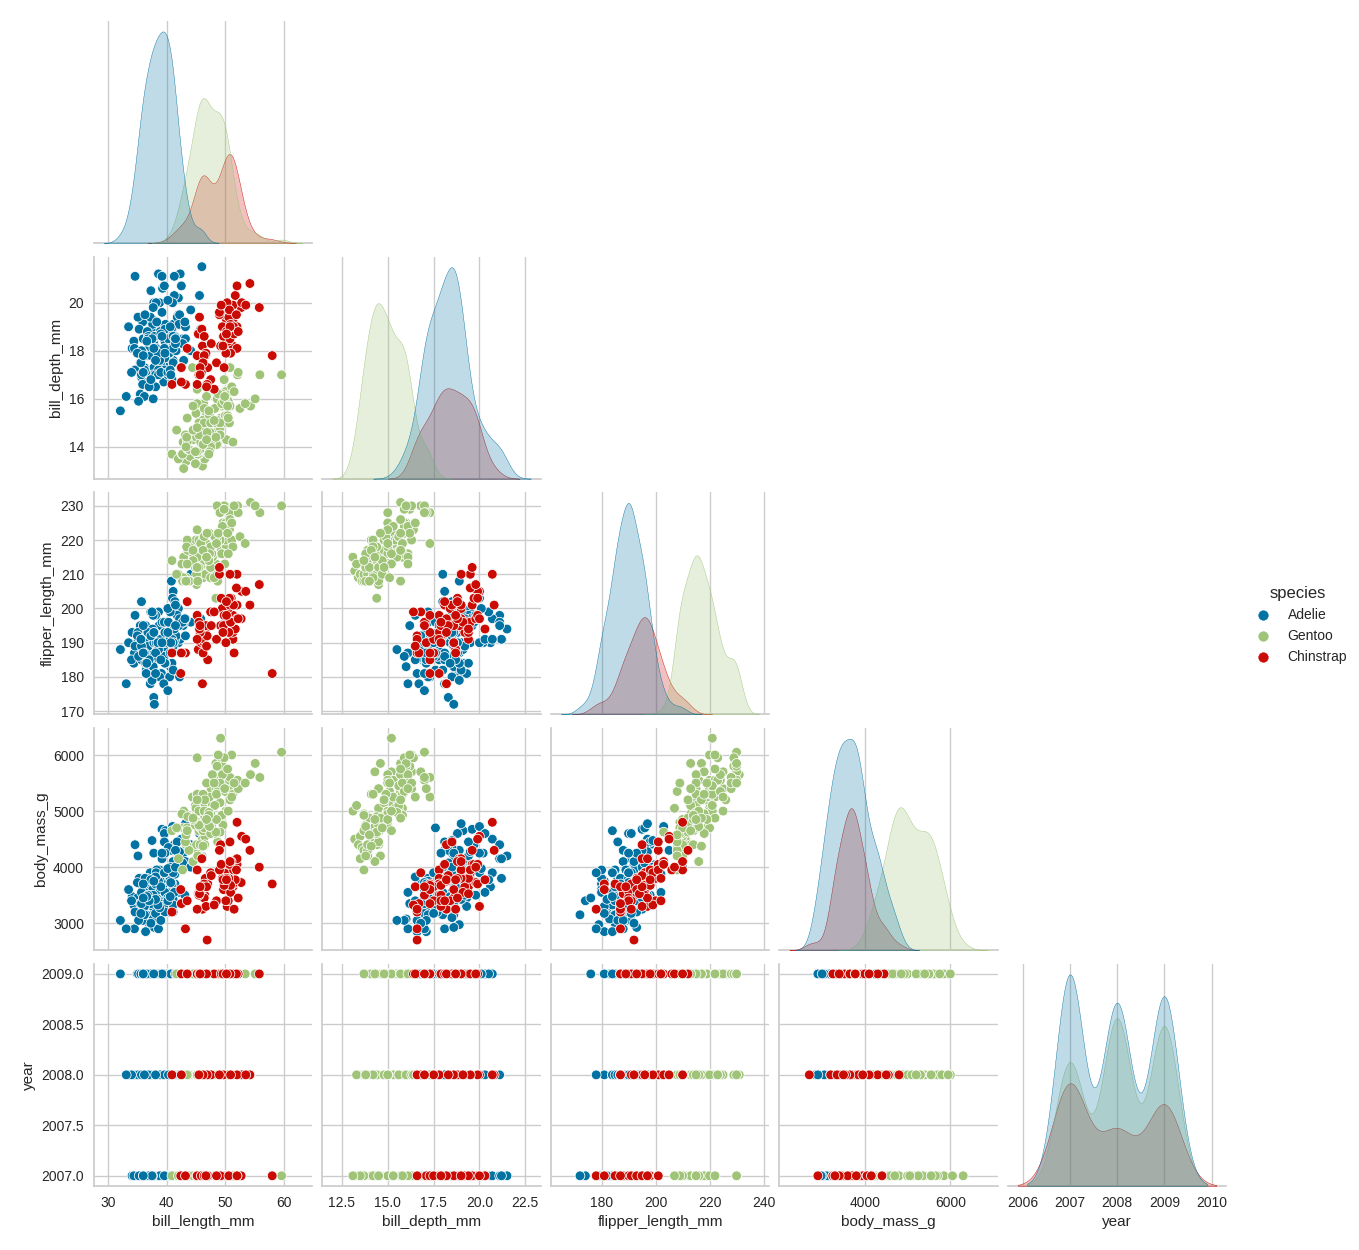
\includegraphics[width=1.0\linewidth]{fig_pairplot}
	\caption{Pairplots}
	\label{fig:pairplots}
\end{figure}

But, unfortunately, the Adelie and Chinstrap separation is not so clear from this chart. On the diagonal of the graph are the histograms for each numeric attribute, and only by the \texttt{bill\_length\_mm} attribute we can see the difference between the Adelie and Chinstrap histograms.

\subsection{Adelie and Chinstrap in more detail}

Let's look at Adelie and Chinstrap in more detail. 
We prepare filtered samples of the data by sex and species (Adelie is additionally filtered by Dream Island, because Chinstrap only lives on it). 
By plotting a histogram for male and another for female shown in Figure \ref{fig:adelieandchinstrap}, we can see that the male sex is perfectly separated, but the female sex has little overlap.

\begin{figure}[h]
	\centering
	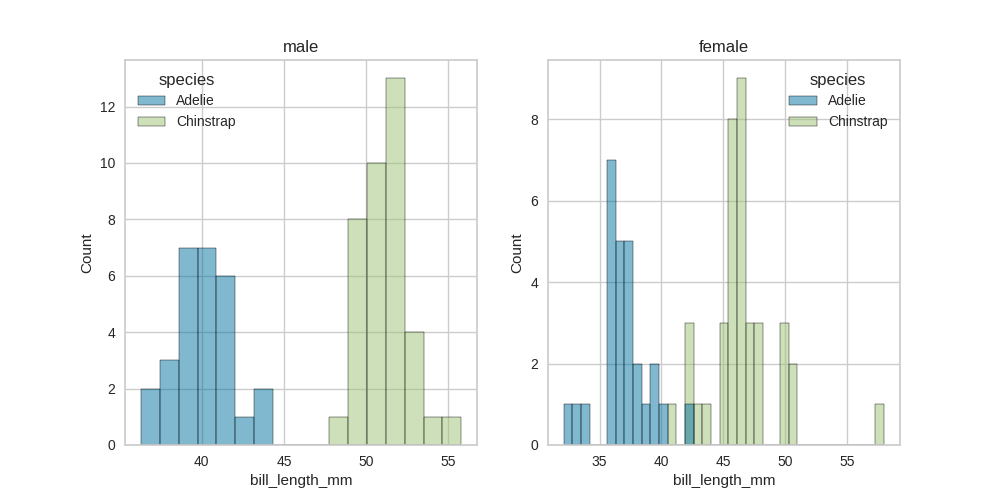
\includegraphics[width=1.0\linewidth]{fig_adelie_chinstrap}
	\caption{Adelie and Chinstrap Histograms}
	\label{fig:adelieandchinstrap}
\end{figure}

For a more detailed analysis of the female gender of Adelie and Chinstrap, we constructed another sns.pairplot, which is shown in Figure \ref{fig:adelieandchinstrappairplot}.
From this matrix of scatter diagrams we could not find features by which the two species could be separated without making a mistake. But the strongest separation was identified in the diagram x = \texttt{bill\_length\_mm} y = \texttt{flipper\_length\_mm}.


\begin{figure}[h]
	\centering
	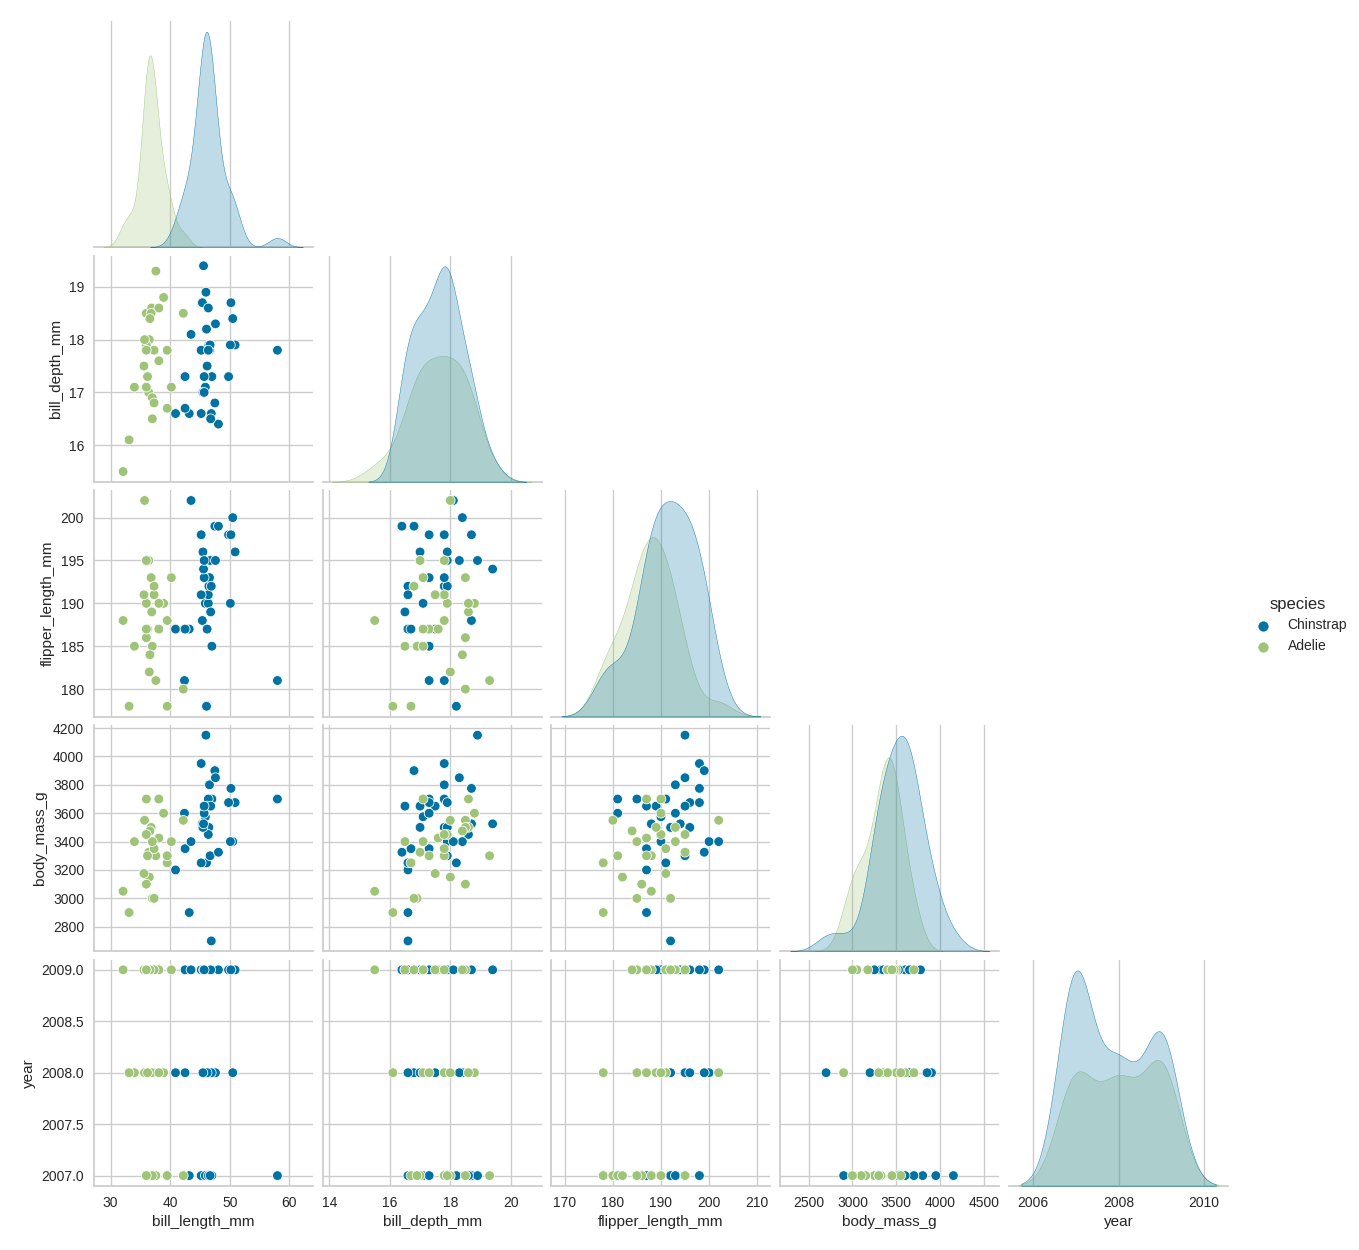
\includegraphics[width=1.0\linewidth]{fig_adelie_chinstrap2}
	\caption{Adelie and Chinstrap Pairplot}
	\label{fig:adelieandchinstrappairplot}
\end{figure}

\section{Modeling}

We have decided to try few different models, mainly the ones which were presented in class,
which means we have done a hyperparameter tuning on
Linear Support Vector Classifier, Decision Tree, Random Forest, Bagging Classifier and Neural Network models.
The values of hyperparameters tried are not that important,
therefore we present only the best hyperparameters, which were found.
These are shown in Table \ref{tbl:hyperparameters}.

\begin{table}[h]
	\centering
	\begin{tabular}{|l|l|}
		\hline
		\textbf{Model} &  \textbf{Hyperparameters} \\
		\hline
		Neural Network & (explained later) \\
		\hline
		Linear Support Vector Classifier & C = $0.5$ \\
		\hline
		Random Forest & criterion = gini \\
		              & max\_depth = None \\
		              & min\_samples\_leaf = $1$ \\
		              & min\_samples\_split = $5$ \\,
		              & n\_estimators = $50$ \\
		\hline
		Bagging Classifier & max\_features = $0.6$, \\
		                   & max\_samples = $0.6$ \\
		\hline
		Decision Tree & criterion = gini, \\
		              & max\_depth = 4 \\
		\hline
	\end{tabular}
	\captionof{table}{The Best Hyperparameters Values Found}\label{tbl:hyperparameters}
\end{table}



\begin{table}[h]
	\centering
\begin{tabular}{|l|r|}
	\hline
	           \textbf{Model} &  \textbf{Accuracy} \\
	\hline
	  Neural Network &  1.000000 \\
	Linear Support Vector Classifier &  0.997260 \\
	   Random Forest &  0.989078 \\
	         Bagging Classifier &  0.989078 \\
	           Decision Tree &  0.978156 \\
	\hline
\end{tabular}
\captionof{table}{Accuracies Of The Models With Best Hyperparameters Values}\label{tbl:accuracies}
\end{table}

The measured accuracies of models with the best hyperparameters found
are shown on Table \ref{tbl:accuracies}.
As we can see, the best accuracy had neural network. That was great also because the assignment explicitly mentions we must save model in h5 format, and we know an easy way how to do it in both Keras (which we use in our neural network model) and scikeras (which is a scikit-learn compatible wrapper for Keras), so we have decided to select neural network as the best model.

The architecture of our neural network model is as follows: The model consists of sequence of Input Layer with $9$ input neurons, followed by a Dense Layer with $16$ neurons and relu activation function, followed by a Dense Layer with $3$ neurons and softmax activation function. The architecture is shown in Figure \ref{fig:neuralnetworkarchitecture}.

\begin{figure}[h]
	\centering
	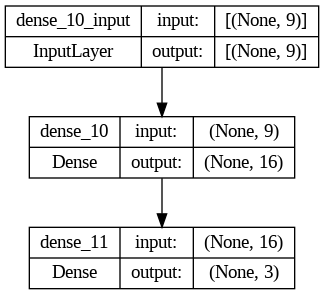
\includegraphics[width=0.5\linewidth]{fig_neural_network_model}
	\caption{The Architecture Of Our Best Neural Network Model}
	\label{fig:neuralnetworkarchitecture}
\end{figure}


\subsection{Model limitations and considerations}

Our model is limited by following factors:

\begin{itemize}
\item The architecture is limited by number of input features, which places a restriction on the number of neurons in input layer, which must be same as number of input features. We do this by setting input\_dim parameter of first Dense layer, however we probably could achieve the same result by using separate Input layer with required number of neurons.
\item The architecture is limited by performed task, which is a multi class classification, which places the following restrictions on the network:

\begin{enumerate}
	\item the number of neurons in output layer must be the same as number of predicted classes
	\item we must use softmax activation function on the last layer, which returns a sequence of predicted class probability scores between 0 and 1 which summs up to 1, where the class with maximum probability score is the class which should be predicted
\end{enumerate}
\end{itemize}

\subsection{Ideas to improve the model}

Model could be improved in such a way that using Dropout layer would prevent overfitting.

\subsection{Choosing the values of hyperparameters}

Values of hyperparameters (such as number of layers or number of neurons in layer) are hardcoded in our model making function and were chosen in such a way that we wanted to start with some small number of layers and neurons and if it would not work well, increase the number of layers or neurons. However, because chosen values worked well, we have not needed to use more complicated networks.

\section{Evaluation}

As we can see from confusion matrix shown at Figure \ref{fig:figconfusionmatrix},
our model achieves 100\% accuracy on the test set. That might look slightly suspicious,
however because we assume perhaps the problem is not as hard as we thought,
we have decided to present this as our result.

\begin{figure}
	\centering
	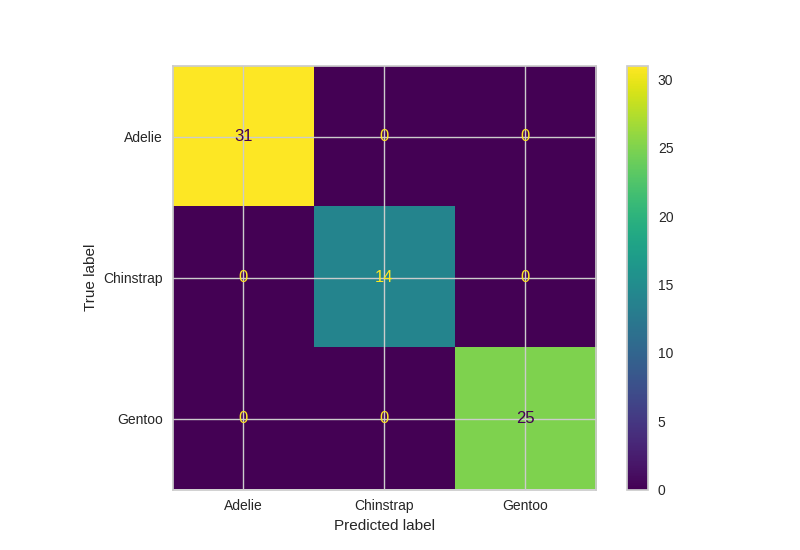
\includegraphics[width=0.7\linewidth]{fig_confusion_matrix}
	\caption{Confusion Matrix}
	\label{fig:figconfusionmatrix}
\end{figure}

\section{Development Environment}

We use Python version 3.9.16 and we also directly use the following packages:

\begin{itemize}
\item \texttt{imblearn} (ver. $0.0$) -- for oversampling using SMOTE method
\item \texttt{matplotlib} (ver. $3.7.1$) -- for visualization
\item \texttt{pandas} (ver. $1.5.3$)-- for working with data in table form
\item \texttt{scikeras} (ver. $0.10.0$) -- contains scikit-learn compatible wrapper which we use
\item \texttt{seaborn} (ver. $0.12.2$) -- for visualization
\item \texttt{scikit-learn} (ver. $1.2.2$) -- for non-neural network models
\item \texttt{tensorflow} (ver. $2.12.0$)-- for neural network models using Keras API
\item \texttt{yellowbrick} (ver. $1.5$)-- for visualization of class prediction error
\end{itemize}

The full list of used libraries in our environment, including their version, can be found on GitHub in the following link (since the list is unreasonably long for display here):

\medskip
\noindent
\url{https://github.com/osmehlik/vse_4it439/blob/master/requirements.txt}

\printbibliography

\end{document}
